\documentclass[a4paper]{article}
\usepackage{graphicx}
\graphicspath{{./figures/}}
\usepackage[italian]{babel}
\usepackage{float}
\usepackage{amsmath, amssymb, braket}
\usepackage{listings}
\usepackage{tikz}
\usetikzlibrary{shapes, arrows, automata, petri, decorations.markings, decorations.pathreplacing, positioning, calc}

\usepackage{hyperref}
\hypersetup{
    colorlinks=false,
}

% Code blocks
\definecolor{codegreen}{rgb}{0,0.6,0}
\definecolor{codegray}{rgb}{0.5,0.5,0.5}
\definecolor{codepurple}{rgb}{0.58,0,0.82}
\definecolor{backcolour}{rgb}{0.95,0.95,0.95}

\lstdefinestyle{mystyle}{
	backgroundcolor=\color{backcolour},
	commentstyle=\color{codegreen},
	keywordstyle=\color{magenta},
	numberstyle=\tiny\color{codegray},
	stringstyle=\color{codepurple},
	basicstyle=\ttfamily\footnotesize,
	breakatwhitespace=false,
	breaklines=true,
	captionpos=b,
	keepspaces=true,
	numbers=left,
	numbersep=5pt,
	showspaces=false,
	showstringspaces=false,
	showtabs=false,
	tabsize=2
}

\lstset{style=mystyle}

\begin{document}

% Title ------------------------------------------------------------------------------
\title{Introduzione alla meccanica quantistica per il quantum computing\\[1ex]
\large Quantum Key Distribution - Protocollo BB84
}

\author{
\vspace{0.8cm}
Università di Verona\\
Imbriani Paolo - VR500437\\
Irimie Fabio - VR501504\\[8ex]
Profssa. Daffara Claudia
}

\begin{figure}
    \centering
    
\includegraphics[width=0.3\textwidth]{UniversityofVerona}
\end{figure}

\maketitle 

\pagebreak
% Title ------------------------------------------------------------------------------

\tableofcontents

\pagebreak

\section{Introduzione}
Fabio e Paolo vogliono instaurare un canale di comunicazione sicuro, in modo da poter
inviare messaggi privati senza che un eventuale attaccante possa intercettarli.
I due si affidano alla crittografia, che permette di codificare i messaggi in modo che
solo il destinatario possa decifrarli.

I due potrebbero utilizzare un metodo classico, come ad esempio il cifrario di Cesare che
prevede di sostituire ogni lettera con una lettera che si trova un certo numero di posizioni
più avanti nell'alfabeto. Ad esempio:
\[
\begin{aligned}
    \text{A} & \rightarrow \text{D} \\
    \text{B} & \rightarrow \text{E} \\
    \text{C} & \rightarrow \text{F} \\
             & \hspace{0.5em}\vdots \\
    \text{Z} & \rightarrow \text{C}
\end{aligned}
\] 
Immaginiamo che Fabio voglia inviare un messaggio a Paolo, per far sì che Paolo
possa decifrare il messaggio, Fabio deve comunicargli la chiave, ovvero il numero
di posizioni da spostare nell'alfabeto. Questo metodo è facilmente intercettabile,
infatti l'attaccante può semplicemente provare tutte le possibili chiavi fino a trovare
quella giusta. Questo tipo di crittografia è detta simmetrica, in quanto sia il mittente
che il destinatario devono possedere la chiave per cifrare e decifrare il messaggio.

\section{Cos'è BB84?}
Per far sì che Fabio e Paolo possano creare un canale di comunicazione sicuro, devono
trovare un modo per scambiarsi la chiave in segreto. Però anche in questo caso, la 
condivisione della chiave deve essere fatta in un canale sicuro, che è il problema
che vogliamo risolvere dal principio!

Il protocollo BB84 è un protocollo di \textit{Quantum Key Distribution} che risolve questo
problema. Se Fabio usasse questo protocollo per trasmettere la chiave a Paolo, loro
potrebbero sapere con \textit{quasi} assoluta certezza se la chiave è stata intercettata o
meno.
\begin{itemize}
  \item Se la chiave \textbf{non} è stata intercettata, Fabio e Paolo avrebbero una chiave
    segreta per instaurare un canale di comunicazione sicuro.

  \item Se la chiave \textbf{è} stata intercettata, Fabio e Paolo possono decidere di non
    utilizzare la chiave e di ripetere il protocollo.
\end{itemize}

\subsection{Requisiti}
Per funzionare, il protocollo BB84 ha bisogno dei seguenti requisiti:
\begin{itemize}
  \item Sia Fabio che Paolo devono avere accesso al proprio computer quantistico.

  \item Devono avere un canale di trasmissione capace di trasmettere qubit. Questo
    potrebbe essere qualche tipo di cavo a fibra ottica capace di trasmettere fotoni
    polarizzati.

  \item Devono avere un canale di comunicazione classico. Siccome è impossibile
    assicurare una sicurezza perfetta, bisogna assumere che qualsiasi canale classico
    può essere intercettato.
\end{itemize}

\subsection{Funzionamento}
I passaggi del protocollo sono i seguenti:
\begin{enumerate}
  \item Fabio crea una stringa casuale di bit, e per ogni bit, lui sceglie casualmente
    una base in cui codificarlo.

  \item Fabio codifica i bit in qubit usando la base scelta, e invia i qubit al computer
    quantistico di Paolo attraverso un canale di comunicazione quantistico.

  \item Anche Paolo sceglie casualmente una base secondo cui decodificare ogni qubit
    ricevuto. Quindi misura ogni qubit nella base che ha scelto.

  \item Fabio utilizza un canale di comunicazione classico per dire a Paolo che basi
    ha scelto per la codifica. Poi comunica anche i primi bit della chiave non codificati.

  \item Paolo analizza questi primi bit per determinare se un intercettatore\\
    (Amos) è riuscito ad entrare nel canale di comunicazione quantistico e intercettare i
    qubit che Fabio gli ha inviato.

  \item Si distinguono due casi:
    \begin{itemize}
    \item Se Amos \textbf{non} ha intercettato i qubit, Fabio e Paolo possono considerare
      tutti i qubit che hanno scelto \textbf{in comune}, cioè con la stessa base, come
      la loro chiave segreta.

    \item Se Amos \textbf{ha} intercettato i qubit, Fabio e Paolo devono ripetere il
      processo da capo.
  \end{itemize}
\end{enumerate}

\section{Scenario concreto}
Prendiamo in considerazione un esempio concreto per capire meglio il protocollo BB84,
in cui Fabio è il mittente e Paolo è il destinatario. Questo esempio è scritto in Python
e utilizza la libreria \texttt{qiskit} per simulare il computer quantistico. Le librerie
da importare sono le seguenti:
\begin{lstlisting}[language=Python]
from qiskit import *
import random
\end{lstlisting}

\subsection{Codifica}
Per prima cosa Fabio deve scegliere una sequenza di bit e basi da utilizzare per
codificare i bit in qubit. Un qubit può essere rappresentato come un vettore sulla sfera
di Bloch, che è una rappresentazione geometrica di uno stato quantistico. Ogni asse
può essere considerato come una possibile base. Quindi se un vettore punta in alto, il
qubit è codificato in $\ket{0}$, se punta in basso è codificato in $\ket{1}$. L'asse
verticale è chiamato \textit{asse \( Z \)}. Nella base \( Z \) possiamo codificare 
lo 0 come $\ket{0}$ (figura \ref{fig:base_z} a sinistra) e l'1 come $\ket{1}$
(figura \ref{fig:base_z} a destra).
\begin{figure}[H]
  \centering
  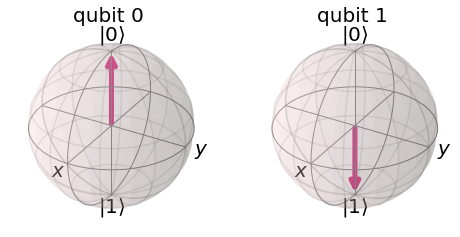
\includegraphics[width=0.6\textwidth]{base_z}
  \caption{Base Z}\label{fig:base_z}
\end{figure}
Un altro modo di codificare i qubit è utilizzare la base \( X \), in cui lo 0 è
rappresentato da $\ket{+}$ (figura \ref{fig:base_x} a sinistra) e l'1 da $\ket{-}$
(figura \ref{fig:base_x} a destra).
\begin{figure}[H]
  \centering
  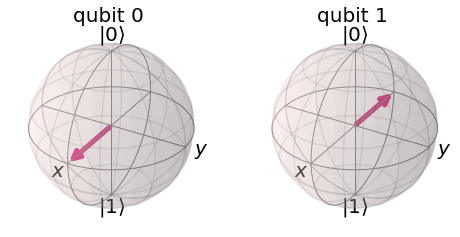
\includegraphics[width=0.6\textwidth]{base_x}
  \caption{Base X}\label{fig:base_x}
\end{figure}

Il primo passo per Fabio è generare casualmente una stringa di bit di lunghezza
arbitraria, ad esempio 300 bit.
\begin{lstlisting}[language=Python]
KEY_LENGTH = 300 # Lunghezza della chiave
random.seed(0)

# Genera una chiave casuale di lunghezza KEY_LENGTH
fabio_bits = ""
for i in range(KEY_LENGTH):
    randBit = random.randint(0, 1) # Numero casuale 0 o 1
    fabio_bits += str(randBit) # Aggiungi il bit alla chiave
    
print("I bit che Fabio invia sono: " + fabio_bits[:10] + "...")
\end{lstlisting}
\begin{lstlisting}
I bit che Fabio invia sono: 1011101010...
\end{lstlisting}
Successivamente Fabio sceglie una base per ogni bit (o in base \( Z \) o in base \( X \)).
\begin{lstlisting}[language=Python]
def generate_random_bases(num_of_bases):
    """Questa funzione seleziona una base casuale per ogni bit"""
    bases_string = ""
    for i in range(num_of_bases):
        randBasis = random.randint(0, 1)

        if randBasis == 0:
            bases_string += "Z" 
        else:
            bases_string += "X"
            
    return bases_string

# Fabio sceglie casualmente una base per ogni bit
fabio_bases = generate_random_bases(KEY_LENGTH)
print("Le basi che Fabio usa sono: " + fabio_bases[:10] + "...")
\end{lstlisting}
\begin{lstlisting}
Le basi che Fabio usa sono: XXZZZXZXZZ...
\end{lstlisting}
Ora Fabio, sul suo computer quantistico, codifica i bit in qubit utilizzando le basi
che ha scelto, creando così una stringa di 300 qubit. Successivamente, Fabio invia i
qubit al computer quantistico di Paolo attraverso un canale di comunicazione
quantistico.

Di default, Qiskit utilizza la base \( Z \) per codificare i qubit e tutti i qubit sono
inizializzati in $\ket{0}$. Per trasformare il qubit in $\ket{1}$ bisogna applicare
una porta \( X \).

Mentre invece, per codificare i qubit in base \( X \) si inizia con i corrispondenti
$\ket{0}$ e $\ket{1}$ e si applica una porta \( H \) (Hadamard) per trasformarli rispettivamente
in $\ket{+}$ e $\ket{-}$.

La tabella delle conversioni è la seguente:
\begin{table}[H]
  \centering
  \begin{tabular}{|c|c|c|c|}
    \hline
    \textbf{Bit} & \textbf{Base} & \textbf{Stato} & \textbf{Porta} \\ \hline
    0 & Z & $\ket{0}$ & - \\ \hline
    1 & Z & $\ket{1}$ & \( X \) \\ \hline
    0 & X & $\ket{+}$ & \( H \) \\ \hline
    1 & X & $\ket{-}$ & \( H,X \) \\ \hline
  \end{tabular}
\end{table}
Usando come riferimento questa tabella, il circuito quantistico per codificare i bit
in qubit è il seguente:
\begin{lstlisting}[language=Python]
def encode(bits, bases):
    """La funzione codifica ogni bit nella base data"""
    
    encoded_qubits = []
    
    for bit, basis in zip(bits, bases):
        # Crea un circuito quantistico per ogni qubit
        qc = QuantumCircuit(1, 1)
        
        # Casi possibili
        if bit=="0" and basis == "Z":
            encoded_qubits.append(qc) # Non serve applicare nessuna porta

        elif bit=="1" and basis == "Z":
            qc.x(0) # Applica porta X
            encoded_qubits.append(qc)

        elif bit=="0" and basis == "X":
            qc.h(0) # Applica porta H
            encoded_qubits.append(qc)

        elif bit=="1" and basis == "X":
            qc.x(0) # Applica porta X
            qc.h(0) # Applica porta H
            encoded_qubits.append(qc)
            
    return (encoded_qubits)


# Codifica i bit di Fabio
encoded_qubits = encode(fabio_bits, alice_bases)

# Print circuits for first 5 qubits.
for i in range(5):
    print(encoded_qubits[i])
print("etc.")
\end{lstlisting}

\subsection{Trasmissione}

Normalmente, i qubit dovrebbero essere inviati attraverso un canale di comunicazione
quantistico, ma essendo che non è possibile avere accesso ad una cosa del genere nel mondo reale,
per semplicità Fabio inserirà i qubit codificati in una lista chiamata \texttt{CANALE\_QUANTISTICO}.
Ovviamente, proprio come un cavo a fibra ottica, il canale quantistico può essere intercettato
da un attaccante.
\begin{lstlisting}[language=Python]
CANALE_QUANTISTICO = encoded_qubits 
\end{lstlisting}

\subsection{Misurazione}

Il passo successivo per Paolo è quello di ricevere i qubit codificati e misurarli.
Prima di tutto, deve scegliere una serie di basi casuali, proprio come ha fatto Fabio in precedenza.
\begin{lstlisting}[language=Python]
paolo_bases = generate_random_bases(KEY_LENGTH)

print("Le basi che Paolo usa sono: " + paolo_bases[:10] + "...")
\end{lstlisting}
\begin{lstlisting}
Le basi che Paolo usa sono: ZXXZZZXZXZ...
\end{lstlisting}
Successivamente, Paolo deve misurare ogni qubit nella base che ha scelto.
In Qiskit, la misurazione di un qubit è rappresentata da una porta \( M \) che
andremo ad inserire per ogni qubit. Tuttavia, dobbiamo stare attenti:
Qiskit non permette di misurare un qubit in una base diversa da quella \( Z \), quindi
dobbiamo prima applicare la porta \( H \) per poter misurare la base \( X \).
\begin{lstlisting}[language=Python]
def measure(qubits, bases):
"""Questa funzione misura ogni qubit nella base corrispondente scelta per esso."""

bits = "" 

for qubit, basis in zip(qubits, bases):

    #  Misurazione dipendente dalla base
    if basis == "Z":
        qubit.measure(0, 0)
    elif basis == "X":
        qubit.h(0)
        qubit.measure(0, 0)

    # Eseguire sul simulatore
    simulator = Aer.get_backend('qasm_simulator')
    result = execute(qubit, backend=simulator, shots=1).result()
    counts = result.get_counts()
    measured_bit = max(counts, key=counts.get) 

    bits += measured_bit
    
return bits
\end{lstlisting}
\begin{lstlisting}[language=Python]
qubits_received = CANALE_QUANTISTICO # Paolo riceve i bit dal canale quantistico
paolo_bits = measure(qubits_received, paolo_bases)

print("I primi bit che Paolo ha ricevuto sono: " + bob_bits[:10] + "...")  
\end{lstlisting}
\begin{lstlisting}
I primi bit che Paolo ha ricevuto sono: 1011101010...
\end{lstlisting}

\subsection{Comparazione}

Ora, Fabio deve comunicare a Paolo le basi che ha scelto per codificare i suoi qubit. 
Lo può fare attraverso qualsiasi canale di comunicazione classico. Il bello di questo protocollo
è che non importa se Amos sa quali basi sono state usate. Fabio potrebbe persino pubblicare queste basi
su un forum pubblico!

\begin{figure}[H]
  \centering
  
\includegraphics[width=1\textwidth]{post}
  \label{fig:post}
\end{figure}

\begin{lstlisting}[language=Python]
CANALE_CLASSICO = fabio_bases # Fabio comunica a Paolo le basi che ha utilizzato
\end{lstlisting}
Per ogni qubit dove Fabio e Paolo hanno scelto basi diverse, c'è un $50\%$ di probabilità
che la misurazione di Paolo ritorni il qubit errato. 
Per esempio, se Fabio invia a Paolo in qubit nello stato $\ket{+}$ (quindi un bit 
0 codificato nella base $X$), e Paolo lo misura nella base \( Z \), c'è una probabilità
nel $50\%$ di ottenere $\ket{0}$ e il $50\%$ di ottenere $\ket{1}$.
Di conseguenza, ogni istanza dove le loro basi non corrispondono è inutile: Paolo deve
trovare le basi che ha in comune con Fabio.
\begin{lstlisting}[language=Python]
common_bases = [i for i in range (KEY_LENGTH) if CANALE_CLASSICO[i] == paolo_bases[i]]

print("Gli indici delle prime dieci basi in comune sono: " + str(common_bases[:10]))
\end{lstlisting}
\begin{lstlisting}
Gli indici delle prime dieci basi in comune sono: [1, 3, 4, 9, 11, 12, 20, 24, 26, 27].
\end{lstlisting}
Ora che Paolo sa le basi in comune, può scartare tutti i bit che non corrispondono con le sue basi
e mantenere solo quelli che invece condividono.
\begin{lstlisting}[language=Python]
paolo_bits = [paolo_bits[index] for index in common_bases]
\end{lstlisting}
Inoltre comunica a Fabio quali basi avevano in comune così che anche lui a sua volta, 
possa scartare il resto dei bit, mantenendo solo quelli che ha in comune con Paolo.
\begin{lstlisting}[language=Python]
CANALE_CLASSICO = common_bases # Paolo comunica a Fabio le basi in comune
\end{lstlisting}
\begin{lstlisting}
fabio_bits = [fabio_bits[index] for index in common_bases]
\end{lstlisting}
Essendo che entrambi mantengono solo i bit misurati con le basi che condividono
\textit{dovrebbero} avere gli stessi bit. Per essere sicuri che questo sia il caso,
Fabio annuncierà i primi bit che ha e Paolo dovrebbe avere gli stessi. 
Ovviamente se Amos provasse ad origliare, anche lui verrebbe a conoscenza dei primi bit,
quindi Fabio e Paolo dovranno successivamente scartarli (solo dopo averli confrontati,
per essere sicuri che abbiano gli stessi bit come previsto). 
\begin{lstlisting}[language=Python]
CANALE_CLASSICO = fabio_bits[:100] 

# Paolo controlla se i primi 100 bit di Fabio corrispondono con i suoi primi 100 bit
if CANALE_CLASSICO == paolo_bits[:100]:
    print("Paolo e Fabio sembrano avere gli stessi bit.")
else:
    print("Almeno un bit e' risultato diverso.")
\end{lstlisting}
\begin{lstlisting}[language=Python]
Paolo e Fabio sembrano avere gli stessi bit.
\end{lstlisting}
Essendo che i primi 100 bit sono uguali, Fabio e Paolo possono essere abbastanza sicuri
che anche i rimanenti bit corrispondono. Ora, devono scartare i primi 100 bit, perchè
Amos potrebbe averli intercettati.
\begin{lstlisting}[language=Python]
fabio_bits = fabio_bits[100:] 
paolo_bits = paolo_bits[100:] 
\end{lstlisting}
A questo punto, i bit rimanenti saranno la \textbf{chiave} che verrà usata per creare
il canale di comunicazione criptato. Ora possono comunicare in libertà senza avere paura che la
loro conversazione venga letta da qualcun altro.
\begin{lstlisting}[language=Python]
key = "" 
for bit in fabio_bits: # O paolo_bits essendo che dovrebbero essere gli stessi.
    key += bit

print("La chiave segreta e':")
print(str(key))

print("\nLa chiave e' lunga" + str(len(key)) + " bit.")
\end{lstlisting}
\begin{lstlisting}
La chiave segreta e':
1011100101011010101001100101101010101111101010001010101110101010001
01000110100101010100101
La chiave e' lunga 90 bit.
\end{lstlisting}

\subsection{Intercettazione} 

Fino ad ora abbiamo considerato che Amos non sia riuscito ad intercettare i qubit, ma cosa
succederebbe se invece ci riuscisse? Vediamo il caso nel dettaglio:\\
Come sempre, Fabio genera una sequenza casuale di basi per codificare i suoi bit.
Successivamente invia questi qubit a Paolo attraverso il canale quantistico.
\begin{lstlisting}[language=Python]
fabio_bits = ""
for i in range(KEY_LENGTH):
    randBit = random.randint(0, 1) 
    fabio_bits += str(randBit) 
 
fabio_bases = generate_random_bases(KEY_LENGTH)

encoded_qubits = encode(fabio_bits, fabio_bases)

CANALE_QUANTISTICO = encoded_qubits
\end{lstlisting}

\subsubsection{Amos ha intercettato i qubit}

Questa volta i qubit vengono intercettati da Amos. 
Vediamo cosa farebbe. Prima di tutto, lui sceglie casualmente una serie di basi
per misurare i qubit (dato che non ha idea di quali basi abbia usato Fabio).
Poi, esegue le misurazioni. Questo è simile a quello che farebbe Paolo normalmente.
\begin{lstlisting}[language=Python]
qubits_intercepted = CANALE_QUANTISTICO # Intercetta i qubit
amos_bases = generate_random_bases(KEY_LENGTH) 
amos_bits = measure(qubits_intercepted, eve_bases) 
\end{lstlisting}
A causa del teorema del no-cloning quantistico, Amos non può semplicemente duplicare esattamente 
i qubit che stanno venendo inviati sul canale quantistico. Di conseguenza, Paolo non riceverà mai 
i qubit originali rendendo ovvio che Amos ha intercettato i qubit.

\subsubsection{Teorema del no-cloning}

Partiamo dalle basi per poter capire al meglio il teorema del no-cloning.\\
Uno stato quantistico $\ket{\psi}$ può essere rappresentato come una combinazione lineare di stati:
\[
\ket{\psi} = \alpha \ket{0} + \beta \ket{1} \]
dove $\alpha$ e $\beta$ sono numeri complessi tali che $|\alpha|^2 + |\beta|^2 = 1$ (normalizzati).
In questo momento si dice che il qubit è in una superposizione di due stati.\\
Quello che dice il teorema del no-cloning è che non esiste un operatore (o trasformazione) universale unitario $U$ tale che
\[\ket{\psi} \otimes \ket{e} \rightarrow \ket{\psi} \otimes \ket{\psi}\]
per qualsiasi input arbitrario (nel nostro caso, sono i bit sono all'interno del canale quantistico) $\ket{\psi}$, dove $\ket{e}$ è uno stato iniziale del sistema da clonare qualsiasi (per esempio $\ket{0})$.\\
In altre parole \textbf{non esiste un processo tale che possa duplicare uno stato quantistico sconosciuto}.

\subsubsection*{Dimostrazione del teorema del no-cloning}

Supponiamo per assurdo che invece \textit{esista} un operatore $U$ tale che
\[U(\ket{\psi} \otimes \ket{e}) = \ket{\psi} \otimes \ket{\psi}\]
\[U(\ket{\phi} \otimes \ket{e}) = \ket{\phi} \otimes \ket{\phi}\]
Ora prendiamo il prodotto interno di entrambi gli output:
\[
\langle \psi | \phi \rangle^2 = \langle \psi | \phi \rangle  \langle \psi | \phi \rangle
\]
Poiché $U$ è un operatore unitario, abbiamo che dovrebbe preservare i prodotti interni.
(Le probabilità totale deve rimanere 1 e le operazioni unitarie devono essere reversibili)
di conseguenza il prodotto interno tra gli stati di input deve essere uguale al prodotto interno tra gli stati di output:
\[\langle \psi | \phi \rangle = \langle \psi | \phi \rangle^2 \]
ricordiamo che:
\[\langle \psi | \phi \rangle = \begin{pmatrix}
  \psi_1 & \psi_2 & \dots & \psi_n 
\end{pmatrix} \begin{pmatrix}
  \phi_1 \\
  \phi_2 \\
  \vdots \\
  \phi_n
\end{pmatrix} = \psi_1\phi_1 + \psi_2\phi_2 + \dots + \psi_n\phi_n\]
L'equazione è vera soltanto se 
\begin{itemize}
  \item $\langle \psi | \phi \rangle = 0$ (stati ortogonali) oppure
  \item $\langle \psi | \phi \rangle = 1$ (stati identici)
\end{itemize}
Questo vuol dire che solo stati ortogonali e stati identici possono essere clonati, ma non stati arbitrari.
Essendo che la maggior parte degli stati quantistici non sono nè ortogonali nè identici, arriviamo ad una contraddizione.
Allora il teorema del no-cloning è vero e non esiste un operatore universale unitario $U$ tale che possa clonare uno stato quantistico sconosciuto. $\square$

\subsubsection{Piano dell'intercettatore}

Per evitare che venga scoperto, Amos deve seguire un piano. Deve inviare una serie di qubit
"sostituti" da mandare a Paolo. Essendo che non ha idea di quali basi abbia usato,
anche lui deve generare una serie di basi casuali. Per semplicità 
assumiamo che Amos usi le stesse basi che ha usato per intercettare i qubit anche per 
codificare i bit di esca.
\begin{lstlisting}[language=Python]
CANALE_QUANTISTICO = encode(amos_bits, amos_bases) # Invia i qubit a Paolo
\end{lstlisting}
Poi Paolo riceve i qubit e li misura nella base che ha scelto. Non sa che Amos li ha intercettati.
Dopodiché Fabio deve comunicare a Paolo che basi ha usato per codificare i qubit. 
Gliele può comunicare attraverso qualsiasi canale di comunicazione classico. Essendo questo canale pubblico
anche Amos saprà le basi che Paolo ha usato.
\begin{lstlisting}
CANALE_CLASSICO = fabio_bases
\end{lstlisting}
Come al solito, Paolo controlla quali basi ha in comune con Fabio. Scarta quelle che non
coincidono e mantiene quelle in comune.
Successivamente comunica a Fabio le basi che ha in comune con lui.

\subsubsection*{Risultato finale}

Essendo che Paolo e Fabio hanno ora solo i qubit misurati con le basi in comune, dovrebbero possedere gli stessi bit.
Per fare sì che questo sia il caso, Fabio annuncerà i primi 100 bit che ha e Paolo dovrebbe avere gli stessi.
\begin{lstlisting}[language=Python]
CANALE_CLASSICO = fabio_bits[:100] 

# Paolo controlla se i primi 100 bit di Fabio corrispondono con i suoi primi 100 bit
if CANALE_CLASSICO == paolo_bits[:100]:
    print("Paolo e Fabio sembrano avere gli stessi bit.")
else:
    print("Almeno un bit e' risultato diverso.")
\end{lstlisting}
\begin{lstlisting}
Almeno un bit e' risultato diverso.
\end{lstlisting}
Dopo aver confrontato i primi 100 bit, Fabio e Paolo
si rendono conto che i loro bit non corrispondono. Assumendo che non ci sia nessun rumore nel canale quantistico
o nei computer quantistici,
Fabio e Paolo sono sicuri che il loro messaggio è stato intercettato.
Di conseguenza decidono di non utilizzare la chiave e di ripetere il protocollo.
La volta successiva potrebbero provare a utilizzare un canale di comunicazione quantistico
diverso, così da confondere Amos.

\pagebreak

\begin{thebibliography}{9}
\bibitem{texbook}
Qiskit Textbook [Internet]. GitHub; 1 Mar. 2025. Disponibile su:\\
\url{https://github.com/Qiskit/textbook/blob/main/notebooks/ch-algorithms/quantum-key-distribution.ipynb}
\end{thebibliography}

 \end{document}
